\section{Transactional Clustering}

Clustering groups objects of a dataset into sets. For numerical data, proximity between objects is measured using distances, typically \textit{Euclidean} or \textit{Manhattan}. However, these measures are not appropriate to carry clustering tasks on categorical attributes, which are used to represent transactional data. The biggest issue is that the way two transactions are deemed \textit{near} each other does not correspond to geometrical proximity.

A simple example makes this concrete. Assume we have four transactions ($T_1$, $T_2$, $T_3$, $T_4$). Transactional data is usually represented with a set of boolean attributes, one for each item, where a value of $1$ marks the presence of the corresponding item and a $0$ marks its absence ($P_1$, $P_2$, $P_3$, $P_4$).

\[
\begin{array}{r c l}
T_1 = \{1,2,3,4\} & \multirow{4}{*}{$\xRightarrow{\text{one-hot encoding}}$} & P_1 = \{1,1,1,1\} \\
T_2 = \{1,2,4\}   &                                                         & P_2 = \{1,1,0,1\} \\
T_3 = \{3\}       &                                                         & P_3 = \{0,0,1,0\} \\
T_4 = \{4\}       &                                                         & P_4 = \{0,0,0,1\} \\
\end{array}
\]

If Euclidean distance were used to measure how far apart these transactions are, we would find the distance between transactions 3 and 4 to be:
\begin{equation*}
    d(P3, P4) = \sqrt{(0)^2 + (0)^2 + (1)^2 + (-1)^2} = \sqrt{2}    
\end{equation*}
The two transactions share no item, so they are completely different, yet the geometric distance stays small. Using a distance metric as a similarity measure for categorical data is therefore not appropriate, and we need algorithms designed to cluster categorical data.

\subsection{K-Modes}
\textbf{K-modes} handles categorical attributes and mirrors K-means. It replaces the Euclidean distance with the mismatch distance, which counts how many elements differ. The algorithm proceeds as follows:
\begin{itemize}
    \item choose $k$ data points at random as representative points;
    \item loop: assign every point to the closest mode;
    \item recompute the mode of each cluster, and repeat until no object changes assignment between two successive iterations (or until some stopping criterion is met).
\end{itemize}

The distance between two records is the number of mismatches between their attributes:
\begin{equation}
    d(X,Y) = \sum_i \delta(x_i, y_i) \qquad
    \delta(x,y) = \begin{cases}
        0 & (x = y) \\
        1 & else
    \end{cases}
\end{equation}
The representative object of a cluster is the mode of the objects it contains, obtained by taking the most frequent value of each attribute: \begin{equation*} f_r(A_j=c_{i,j} | X_i) = \dfrac{n_{c_{i,j}}}{n}
\end{equation*}

\paragraph{K-modes Optimization Model}
\begin{align*}
    \min\quad P(W,Q) = &\sum_{i}^k \sum_{j}^n w_{i,j} d(X_j, Q_i)\\
    \text{subject to}\quad \sum_{i}^k w_{i,j} = &1 &  1 \leq j \leq n \\
    w_{i,j} \in& \{0,1\} & 1 \leq i \leq k && 1 \leq j \leq n 
\end{align*}
\begin{itemize}
    \item $Q = \left\{Q_1,\dots,Q_k\right\}$ is the set of representative objects (mode) for the clusters.
    \item $d(X_j, Q_i)$ is a distance function for objects in the data.
    \item $W$ is a matrix $k \times n$; $w_{i,j}= 1$ if object $j$ belongs to cluster $i$, 0 otherwise;
    \item $X=\{X_1,..,X_n\}$ is the dataset of objects and $X_i=[x_1,..,x_m]$ is a single object.
\end{itemize}

\paragraph{Initialization Issue} Every run can return a different result, because the initial modes are chosen at random. Each run is cheap, so we run the algorithm many times and keep the solution with the smallest error.

\subsection{RObust Clustering Using Link (ROCK)}
\textbf{ROCK} is a \textbf{hierarchical} algorithm that uses \textbf{neighborhoods} and \textbf{links to clusters} (instead of the classical distance) to define closeness between \textit{transactional data}. It behaves like the agglomerative algorithm, but works only on transactional data in its pure form. Neighborhoods are computed locally, links are computed globally. The algorithm is very slow and splits into three parts:
\begin{enumerate}
    \item \textbf{A random sample is drawn from the dataset.} A sample of points is extracted uniformly (\textit{random sampling is the fastest}) and used to form the clusters in place of the whole dataset, so the algorithm can run on a large dataset while still producing an accurate enough clustering.

    \item \textbf{Agglomerative hierarchical clustering runs on the sample.} It starts by assigning each point to a singleton cluster, then computes the similarity measure for all pairs of clusters and merges the two \textit{closest} objects. These steps repeat until some stopping condition is met, usually until $k$ clusters are formed.

    Two objects $A$ and $B$ are \textbf{neighbors} if their similarity is greater than or equal to some hyperparameter threshold $\theta$, chosen between 0 and 1:
    \begin{equation*}
        A \in N_B \land B \in N_A \iff sim(A,B) \geq \theta \,
    \end{equation*}
    ROCK uses the Jaccard coefficient as the similarity and treats a point as a neighbor of itself:
    \begin{equation*}
        sim(A,B) = \dfrac{|A \cap B|}{|A \cup B|}
    \end{equation*}
A \textbf{link} is calculated as the number of common neighbors between two objects:
    \begin{equation*}
        link(A,B) = |N_A \cap N_B|
    \end{equation*}
    A higher link value means a higher probability that the two objects belong to the same group, since they share neighbors. Similarity captures a local relationship, while the link captures global information.

    \item \textbf{The entire dataset is labeled by assigning each object to a cluster.} A random sample is selected from each cluster, and each point $p$ in the original dataset is assigned to the cluster $i$ in whose sample $p$ has the maximum number of neighbors.
\end{enumerate}

\paragraph{Criterion Function}
The best clusters are the ones that maximize the criterion function:
\begin{align*}
    &E_l = \sum_{i=1}^k n_i \sum_{p_q,p_r \in C_i} \dfrac{link(p_q, p_r)}{n_i^{1 + 2 f(\theta)}} \,, \\
    & f(\theta) = \dfrac{1-\theta}{1+\theta}
\end{align*}
where $n_i$ is the size of cluster $C_i$, $k$ the number of clusters, and $\theta$ the similarity threshold. Dividing by the expected number of links between pairs of objects in cluster $C_i$ penalizes assigning objects that share few links to the same cluster. At each merging step, the two clusters merged are the ones that maximize:
\begin{equation*}
    g(C_i, C_j) = \frac{\overbrace{link(C_i, C_j)}^\text{number of cross links between clusters $i$ and $j$}}{\underbrace{(n_i + n_j)^{1+2f(\theta)} - n_i^{1+2f(\theta)} - n_j^{1+2f(\theta)}}_{\text{expected number of cross links between clusters $i$ and $j$}}} \qquad \text{goodness measure}
\end{equation*}

\subsection{CLOPE (Clustering with sLOPE)}

CLOPE is a clustering algorithm efficient on high-dimensional data. It relies on a purely \textit{global criterion function} that raises the intra-cluster overlap of transactions by increasing the height-to-width ratio of the cluster histogram. It suits large datasets with many unique items, since it stores the data as an array instead of a binary matrix.

For each cluster, the width is the number of distinct items, and the height is the ratio between the total number of (non-unique) items and the width.
\begin{figure}[h]
    \centering
    \begin{minipage}{0.3\textwidth}
    \centering
    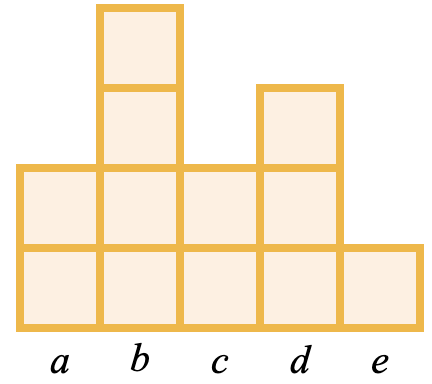
\includegraphics[width=0.3\linewidth]{img/CLOPE.png}
    \begin{equation*}
        C_i = \{abcd, bcd, ab, bde\}
    \end{equation*}
    \end{minipage}
    \begin{minipage}{0.49\textwidth}
        \begin{gather*}
            W(C_i) = 5 \\
            S(C_i) = 12 \\
            H(C_i) = \dfrac{12}{5} = 2.4
        \end{gather*}
    \end{minipage}
\end{figure} \\
A higher height/width ratio means greater item overlap. The goodness of a clustering is measured as the \textbf{gradient} of each cluster:
\begin{equation}
    Profit_r(C) = \dfrac{\sum_{i=1}^k \dfrac{S(C_i)}{W(C_i)^r} \times |C_i|}{\sum_{i=1}^k |C_i|}
\end{equation}
\paragraph{Repulsion $r$} This is a hyperparameter. For higher values of $r$, transactions in the same cluster must share a large fraction of common items; for lower values they may share fewer items, which helps with sparse databases.

The algorithm first adds each transaction either to a new cluster or to the existing cluster that maximizes the profit. It then checks, for each transaction, whether moving it to a different cluster improves the profit, and repeats this step until no move improves the profit.

\subsection{TX-Means}
TX-Means is a parameter-free transactional clustering algorithm useful for partitioning data drawn from a very large number of different datasets. It finds a representative transaction for each cluster, which summarizes the pattern shared by the elements of that cluster. Like X-Means, it starts with a single cluster holding all the objects in the dataset, then decides how to split it recursively into subpartitions using the BIC (Bayesian Information Criterion).

\begin{algorithm}
\caption{TX-Means pseudocode.}
\begin{algorithmic}[1]
    \State $r$ = \texttt{getRepr}($B$)  \quad  \Comment{Get representative basket of entire set of baskets}
    \State $r$ is added to queue $Q$
    \While{$Q \neq \emptyset$} \Comment{split each cluster in $Q$}
        \State $C, r$ are extracted from $Q$
        \State Common items are removed from $C$ and $r$ \Comment{Common items not meaningful}
        \State $C1,C2,r1,r2$ = \texttt{bisectBasket}($C$)
        \If{$BIC(C1,C2,r1,r2) > BIC(C,r)$}  \Comment{BIC comparison}
            \State Add $C1,C2,r1,r2$ to $Q$ \Comment{Split accepted: add $C_1$ and $C_2$ in $Q$}
        \Else
            \State Add $C, r$ to result \Comment{Split not accepted: we have a result}
        \EndIf
    \EndWhile
    \State Return result
\end{algorithmic}
\end{algorithm} 

\begin{algorithm}
\caption{\texttt{getRepr} pseudocode.}
\begin{algorithmic}[1]
    \State $I$ = set of items not shared among all baskets in $B$ \Comment{Items not common to all}
    \State $r$ = set of items in common to all baskets in $B$ \Comment{Representative with common items}
    \State Calculate frequencies of items in $I$ \Comment{Count occurrences of each item}
    \State $i = 0$, $d_0 = \inf$ \Comment{Initialize iteration counter and distance}
    \While{$I \neq \emptyset$} \Comment{Continue until no items left to consider}
        \State $i = i + 1$ \Comment{Increment iteration counter}
        \State Add the items in $I$ with maximum frequency to $r$
        \State Calculate $d_i(r,B)$ via Jaccard distance \Comment{Measure how well r represents B}
        \If{$d_i \geq d_{i-1}$} \Comment{Check if distance increased (worse representation)}
            \State Return $r$ \Comment{Stop if adding items worsened representation}
        \Else
            \State Remove from $I$ items with maximum frequency
        \EndIf
    \EndWhile 
    \State Return $r$ \Comment{Return final representative basket}
\end{algorithmic}
\end{algorithm}

\begin{algorithm}
\caption{\texttt{bisectBasket} pseudocode.}
\begin{algorithmic}[1]
    \State $SSE = \inf$
    \State Select two random baskets $r1,r2$
    \While{True}
        \State $C1,C2$ = clusters obtained by assigning baskets to either $r1$ or $r2$
        \State $r1_{new}$ = \texttt{getRepr}($C1$)
        \State $r2_{new}$ = \texttt{getRepr}($C2$)
        \State $SSE_{new} = SSE(C1,C2,r1_{new},r2_{new})$
        \If{$SSE_{new} \geq SSE$}
            \State Return $C1,C2,r1,r2$ \quad \Comment{If the next step bring us to a worst situation we stop}
        \EndIf
        \State $r1 = r1_{new}$
        \State $r2 = r2_{new}$
        \State $SSE = SSE_{new}$
    \EndWhile
\end{algorithmic}
\end{algorithm}
\paragraph{Sampling Strategy}
TX-Means also scales through the following sampling strategy:
\begin{itemize}
    \item select a random subset $S$ of the baskets in $B$;
    \item run TX-Means on the subset $S$ to obtain clusters $C$ and representative baskets $R$;
    \item assign the remaining baskets $B/S$ to the clusters $C$ with a nearest-neighbor (NN) approach against the representative baskets $R$.
\end{itemize}
